\documentclass[a4paper,9pt,twocolumn]{extarticle}
\usepackage[utf8]{inputenc}
\usepackage{graphicx}
\usepackage[center, font=small]{caption}
\usepackage[english]{babel}
\usepackage[top=2.5cm, bottom=2.5cm, left=2cm, right=2cm]{geometry}

%---------------------------------------------
% Font packages
%---------------------------------------------
% \usepackage{lmodern}
% \usepackage{concmath}
% \usepackage{cmbright}
% \usepackage{kpfonts}
% \usepackage[adobe-utopia]{mathdesign}
\usepackage{fouriernc}
\usepackage[T1]{fontenc}

%---------------------------------------------
% Math environment packages & command
%---------------------------------------------
\usepackage{amsmath}
\usepackage{amssymb}
\usepackage{array}
% \usepackage{mathrsfs}
\usepackage{array}
% \def\sgn{\mathop{\rm sgn}\nolimits} 
% \usepackage{bbm}
\usepackage{schemabloc}

%---------------------------------------------
% item option
%---------------------------------------------
\renewcommand{\labelitemi}{-}

%---------------------------------------------
%HEADER & FOOTER
%---------------------------------------------
\usepackage{fancyhdr}
\pagestyle{fancy}

\renewcommand{\headrulewidth}{.15pt}
\fancyhead[C]{{\textsc{The Four-Tank Process}}} 
\fancyhead[L]{Page \thepage \ of \pageref{LastPage}}
\fancyhead[R]{EL2520}

\renewcommand{\footrulewidth}{.15pt}
\fancyfoot[C]{$\ast\phantom{a}\thepage\phantom{a}\ast$} 
% \fancyfoot[L]{\emph{David, Demeulemeester, Masson, Pouech}}
\fancyfoot[R]{EE -- Automatic Control}

\usepackage{lastpage}

%---------------------------------------------
% two column option
%---------------------------------------------
\setlength{\columnsep}{0.7cm}

%---------------------------------------------
% Table of content
%---------------------------------------------
\usepackage[colorlinks,linkcolor=black, citecolor=black]{hyperref}

%---------------------------------------------
% Opening
%---------------------------------------------
\title{Control Theory and Practice \\ Advanced Course \\ \textsc{The Four-Tank Process}}
\author{Jean-Alix \textsc{David}, Kilian \textsc{Demeulemeester}, Clément \textsc{Masson}, Jeremy \textsc{Pouech} \\ \texttt{\{jadavid,kiliande,cmasson,pouech\}@kth.se}}

%---------------------------------------------
% Numerotation Handling
%---------------------------------------------
\setcounter{section}{1}
\usepackage[explicit]{titlesec}
% \titleformat{<command>}[<shape>]{<format>}{<label>}{<sep>}{<before>}[<after>]
\titleformat{\subsubsection}[hang]{\Large\normalsize\bfseries\centering}%
    {}{4pt}%
    {\dotfill\hspace{0.5cm}\emph{#1 \arabic{section}.\arabic{subsection}.\arabic{subsubsection}}\hspace{0.5cm}\dotfill} 

    \titleformat{\paragraph}[hang]{\footnotesize\bfseries\centering}{}{4pt}{\emph{#1}}
    %\titleformat{\paragraph}[hang]{\footnotesize\bfseries}{}{4pt}{\dotfill\hspace{0.5cm}\emph{#1}\hspace{0.5cm}\dotfill}
%---------------------------------------------
% Dummy text
%---------------------------------------------
\usepackage{lipsum}

%---------------------------------------------
% Item package option 
%---------------------------------------------
%\usepackage[shortlabels]{enumitem}
\newenvironment{shortitemize}{
    \begin{itemize}
        \setlength{\itemsep}{0pt}
        \setlength{\parskip}{0pt}
        \setlength{\parsep}{0pt}
    }{\end{itemize}}

\begin{document}

% Indent length
\setlength\parindent{0em}

\maketitle

%\tableofcontents

\begin{bfseries}
\emph{Abstract} -- Blablabla ! 
\end{bfseries}


\section{Laboratory occasion 1}

\subsection{Modeling}

In the following exercices we will construct a physical model of the four-tank process.

\subsubsection{Exercise} 

We have the following equation for each tank:
\begin{equation}
A \frac{dh}{dt} = q_{in} - q_{out} 
\label{floweq}
\end{equation}

The following table establish $q_{in}$ and $q_{out}$ for each tank:
$$
\begin{array}{|c|cc|}
    \hline
    & q_{in} & q_{out} \\
    \hline
    \text{Tank} 1 & \gamma_1k_1u_1+a_3\sqrt{2gh_3} & a_1\sqrt{2gh_1} \\
    \text{Tank} 2 & \gamma_2k_2u_2+a_4\sqrt{2gh_4} & a_2\sqrt{2gh_2} \\
    \text{Tank} 3 & (1-\gamma_2)k_2u_2 & a_3\sqrt{2gh_3} \\ 
    \text{Tank} 4 & (1-\gamma_1)k_1u_1 & a_4\sqrt{2gh_4} \\ 
    \hline
\end{array}
$$

Therefore according to equation (\ref{floweq}): 
$$
    \begin{array}{rcl}
    A_1 \frac{dh_1}{dt} & = &
        \gamma_1k_1u_1+a_3\sqrt{2gh_3} - a_1\sqrt{2gh_1} \\
    A_2 \frac{dh_2}{dt} & = &
        \gamma_2k_2u_2+a_4\sqrt{2gh_4} - a_2\sqrt{2gh_2} \\
    A_3 \frac{dh_3}{dt} & = &
        (1-\gamma_2)k_2u_2 - a_3\sqrt{2gh_3} \\ 
    A_4 \frac{dh_4}{dt} & = &
    (1-\gamma_1)k_1u_1 - a_4\sqrt{2gh_4} \\ 
    \end{array}
$$

And finally:
\begin{equation}
    \boxed{
        \begin{array}{rcl}
    \frac{dh_1}{dt} & = &
            - \frac{a_1}{A_1}\sqrt{2gh_1} + \frac{a_3}{A_1}\sqrt{2gh_3} + \frac{\gamma_1k_1}{A_1}u_1\\ 

    \frac{dh_2}{dt} & = &
            - \frac{a_2}{A_2}\sqrt{2gh_2} + \frac{a_4}{A_2}\sqrt{2gh_4} + \frac{\gamma_2k_2}{A_2}u_2\\ 

    \frac{dh_3}{dt} & = &
            -\frac{a_3}{A_3}\sqrt{2gh_3}+\frac{(1-\gamma_2)k_2}{A_3}u_2 \\ 

    \frac{dh_4}{dt} & = &
            -\frac{a_4}{A_4}\sqrt{2gh_4}+\frac{(1-\gamma_1)k_1}{A_4}u_1 \\ 
        \end{array}
    \label{tanksyseq}
}
\end{equation}

\subsubsection{Exercise} \lipsum[1-2]

\subsubsection{Exercise} \lipsum[1-2]

\subsubsection{Exercise} \lipsum[1-2]

\subsubsection{Exercise}

The zeros of $G(s)$ are given by the zeros of $P(s)$ in the following expression:
$$
\det G(s) = \frac{k_1k_2c_1c_2}{\prod_{i=1}^{4} (1 + s T_i)}
\underbrace{\left[ (1+sT_3)(1+sT_4) - \frac{(1-\gamma_1)(1 - \gamma_2)}{\gamma_1\gamma2}\right]}_{P(s)}
$$

$P$ is a second degree polynom. Its discrimant is:

$$
\Delta_P = (T_3+T_4)^2 - 4\frac{T_3T_4}{\gamma_1\gamma_2}(\gamma_1+\gamma_2-1) 
$$

    $$\ast \phantom{aa} \text{If} \phantom{a} 0 < \gamma_1 + \gamma_2 \leq 1$$
In that case $\gamma_1 + \gamma_2 - 1 \leq 0$. 

Therefore
$\Delta_P \geq 0$.

The roots of $P$ are given by:
$$
p_{1,2} = \frac{-(T_3+T_4) \pm_\text{\tiny{2}}^\text{\tiny{1}} \sqrt{\Delta_P}}{2T_3T_4}
$$

And 
\begin{multline*}
    -4\frac{T_3T_4}{\gamma_1\gamma_2}(\gamma_1+\gamma_2-1) \geq 0 \\ \Leftrightarrow \Delta_P \geq (T_3+T_4)^2 \Leftrightarrow \sqrt{\Delta_P}\geq (T_3+T_4)$$
\end{multline*}
Leading to:
$$
p_1 = \frac{-(T_3+T_4) + \sqrt{\Delta_P}}{2T_3T_4} \geq 0
$$

The system is non-minimum phase.


    $$\ast \phantom{aa} \text{If} \phantom{a} 1 < \gamma_1 + \gamma_2 \leq 2$$
In that case $\gamma_1+\gamma_2 -1 > 0$.

Therefore
$\Delta_P < 0$.

The real-part of the roots of $P$ is:
$$
\Re(p_{1,2}) = -\frac{(T_3+T_4)}{2T_3T_4} \leq 0
$$

The system is minimum phase.

\paragraph{Recap}

We prooved the following:
$$
\begin{array}{rcl}
    0 < \gamma_1 + \gamma_2 \leq 1 & \Rightarrow & \text{Minimum phase system} \\
    1 < \gamma_1 + \gamma_2 \leq 2 & \Rightarrow & \text{Non-minimum phase system} \\
\end{array}
$$

\subsubsection{Exercise} 

The RGA of the system at frequency 0 is:
$$
\text{RGA}(G(0)) = G(0).\ast[G^{-1}(0)]^T 
$$

With:

\begin{equation*}
    G(0) =
\left[
    \begin{array}{cc}
        \gamma_1k_1c_1 & (1-\gamma_2)k_2c_1 \\
        (1-\gamma_1)k_1c_2 & \gamma_2k_2c_2 \\
    \end{array}
\right]
\end{equation*}
\begin{multline*}
[G^{-1}(0)]^T = \\
\frac{1}{k_1k_2c_1c_2(\gamma_1+\gamma_2-1)}
\left[
    \begin{array}{cc}
        \gamma_2k_2c_2 & -(1-\gamma_1)k_1c_2 \\
        -(1-\gamma_2)k_2c_1 & \gamma_1k_1c_1 \\
    \end{array}
\right]\\
\end{multline*}
Leading to:
\begin{multline*}
    \text{RGA}(G(0)) =\\ 
\frac{1}{\gamma_1+\gamma_2-1}
\left[
    \begin{array}{cc}
        \gamma_1\gamma_2 & -(1-\gamma_1)(1-\gamma_2) \\
        -(1-\gamma_1)(1-\gamma_2) & \gamma_1\gamma_2 \\
    \end{array}
\right]
\end{multline*}

\begin{equation}
    \boxed{
    \text{RGA}(G(0)) =
    \left[
        \begin{array}{cc}
            \lambda & 1 - \lambda \\
            1 - \lambda & \lambda
        \end{array}
    \right]
}
\end{equation}

Where $\lambda = \frac{\gamma_1\gamma_2}{\gamma_1+\gamma_2-1}$.

\paragraph{Minimum phase case}
In that case $\gamma_1 = \gamma_2 = .625$. Thus:
$$
\text{RGA}(G_{m}(0)) =
    \left[
        \begin{array}{cc}
            1.5625 & -0.5625 \\
            -0.5625 & 1.5625
        \end{array}
    \right]
$$

\paragraph{Non-minimum phase case}
In that case $\gamma_1 = \gamma_2 = .325$. Thus:
$$
\text{RGA}(G_{nm}(0)) =
    \left[
        \begin{array}{cc}
            -0.5625 & 1.5625 \\
            1.5625 & -0.5625
        \end{array}
    \right]
$$

\subsubsection{Exercise}

The following procedure will be used to determine $k_1$ and $k_2$ $\left[\frac{cm^3}{s.V}\right]$:

\begin{shortitemize}
    \item Bloc every holes of the tanks (therefore $a_i = 0, \forall i$)
        In that situation we have the following equation:
            $$
            h_1(t) = \frac{\gamma_1k_1}{A_1}u_1(100\%)t \\
            $$
            $$
            h_2(t) = \frac{\gamma_2k_2}{A_2}u_2(100\%)t \\
            $$
    \item Set the two pump to 100\% of the control signals,
    \item Measure the evolution of $y_1$ and $y_2$,
    \item Using linear regression on the curves, determine $k_1$ and $k_2$.
\end{shortitemize}

Table \ref{parameterDetermination} sum up the parameters determination.


\subsubsection{Exercise} 

The following procedure were used to determine $a_i \left[m^2\right], \forall i$:

\begin{shortitemize}
    \item Set up the correct outlets for each tank in order to be in minimum case or non-minimum case,
    \item DO SOME SHIT
\end{shortitemize}

\begin{table}[h!b]
    \centering
    \begin{tabular}{|r|l|c|}
        \hline
        \multicolumn{3}{|c|}{Parameters}\\
        \hline
        $k_1$           & $4.0674$ & \multirow{2}{*}{$\frac{cm^3}{s.V}$}  \\
        $k_2$           & $3.7167$  & \\
        \hline 
        $a_1$           & $0.1726$  & \multirow{6}{*}{$m^2$}  \\
        $a_2$           & $0.1479$  & \\
        $a_{3,min}$     & $0.0856$  & \\
        $a_{4,min}$     & $0.0728$  & \\
        $a_{3,nonmin}$  &   & \\
        $a_{4,nonmin}$  &   & \\
        \hline
    \end{tabular}
    \caption{Parameter values}
    \label{parameterDetermination}
\end{table}



% \subsection{Manual control}

\subsubsection{Exercise}

Since the method used in exercise 2.1.8 is based on the measure of $h_{1\leq i \leq 4}^0$ with the pumps on $50\%$, the levels are in accordance with the calculations. 
(result valid for both minimum phase case and non-minimum phase case.)

% \subsubsection{Exercise} 

\paragraph{Minimum phase case}

Figure \ref{steprepmin} shows the step response from one input at a time.

\begin{figure}[h!t]
        \centering
        \begin{subfigure}[b]{0.45\columnwidth}
                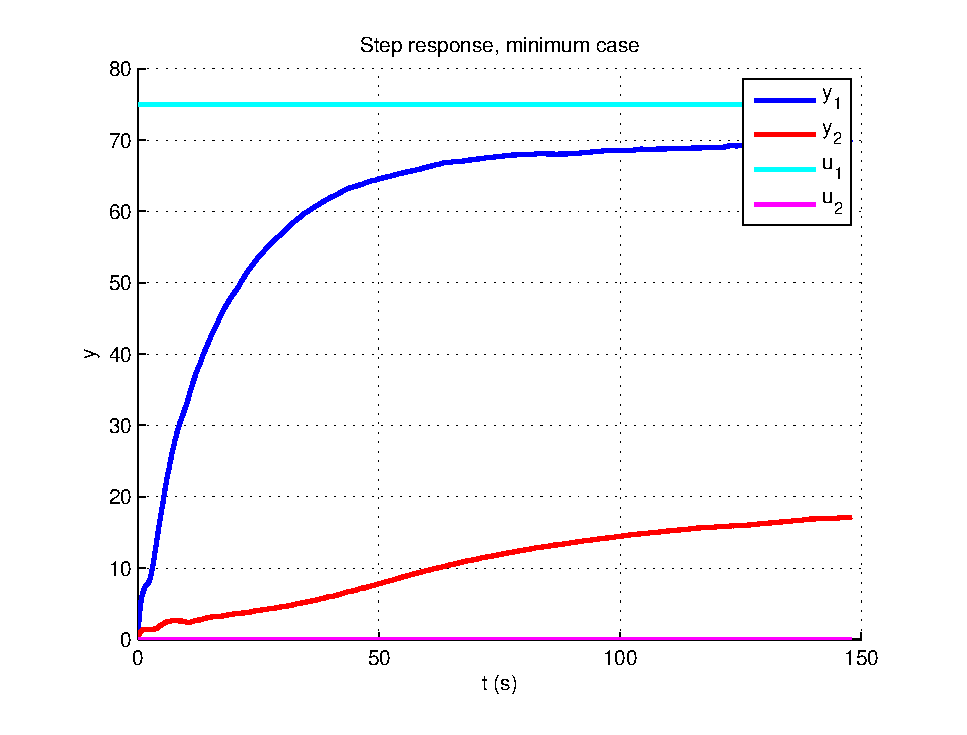
\includegraphics[width=\columnwidth]{fig/steprepmin75_0.eps}
                \caption{$u_1 = 75\%, u_2 = 0\%$}
        \end{subfigure}
        \begin{subfigure}[b]{0.45\columnwidth}
                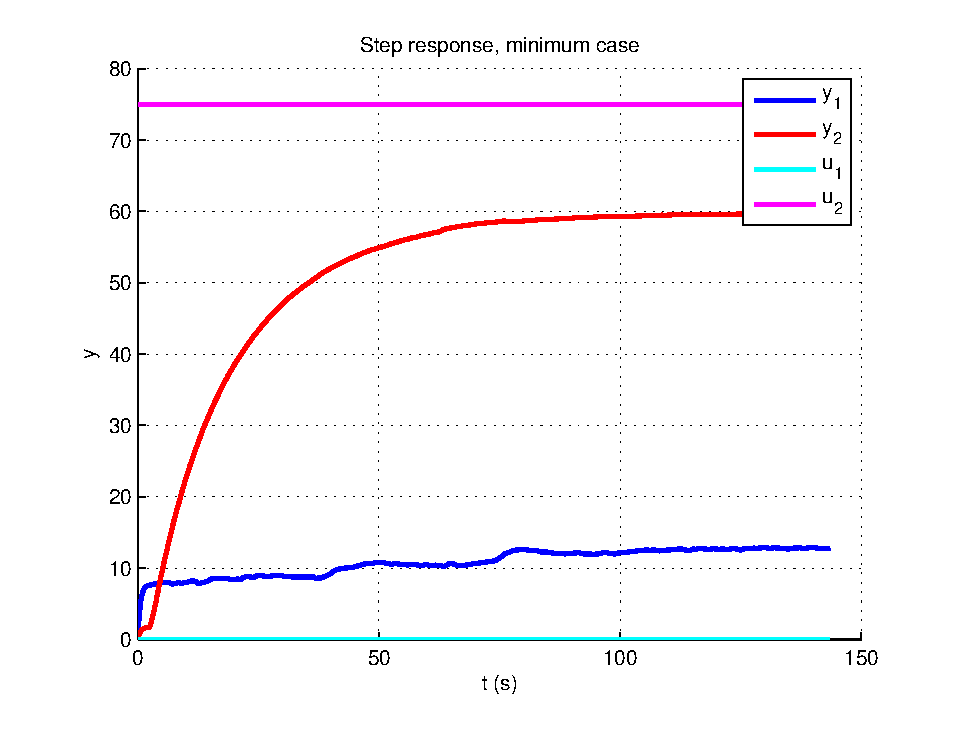
\includegraphics[width=\columnwidth]{fig/steprepmin0_75.eps}
                \caption{$u_1 = 0\%, u_2 = 75\%$}
        \end{subfigure}
        \caption{Step response from one input at a time \\ for the minimum phase case} 
        \label{steprepmin}
\end{figure}

\paragraph{Non-minimum phase case} 

Figure \ref{steprepnonmin} shows the step response from one input at a time.

\begin{figure}[h!t]
        \centering
        \begin{subfigure}[b]{0.45\columnwidth}
                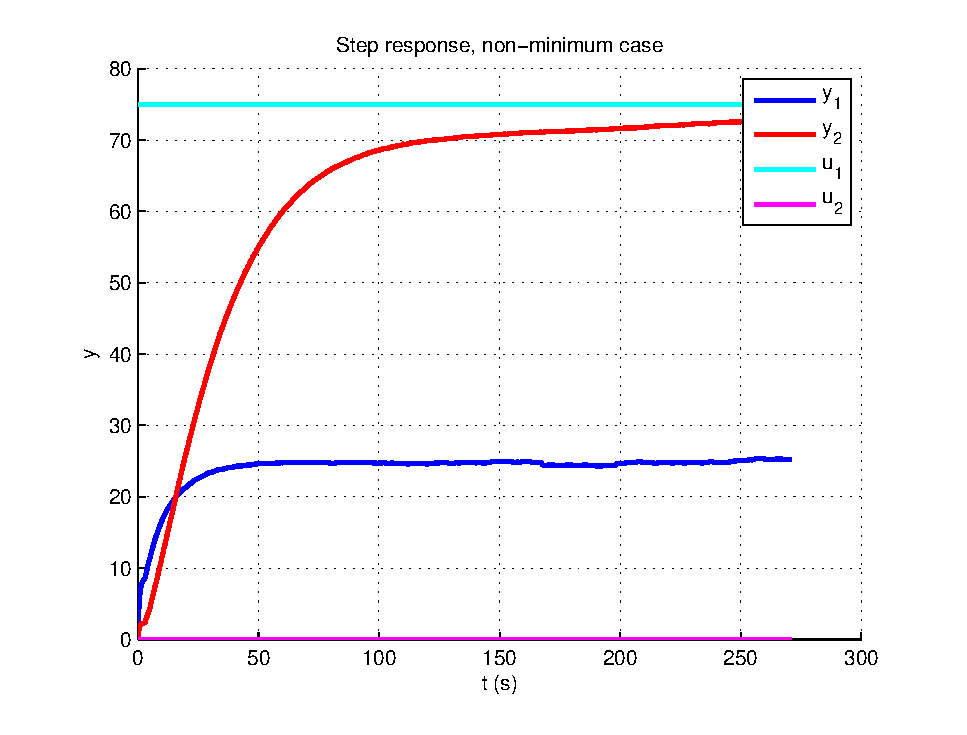
\includegraphics[width=\columnwidth]{fig/steprepnonmin0_75.eps}
                \caption{$u_1 = 75\%, u_2 = 0\%$}
        \end{subfigure}
        \begin{subfigure}[b]{0.45\columnwidth}
                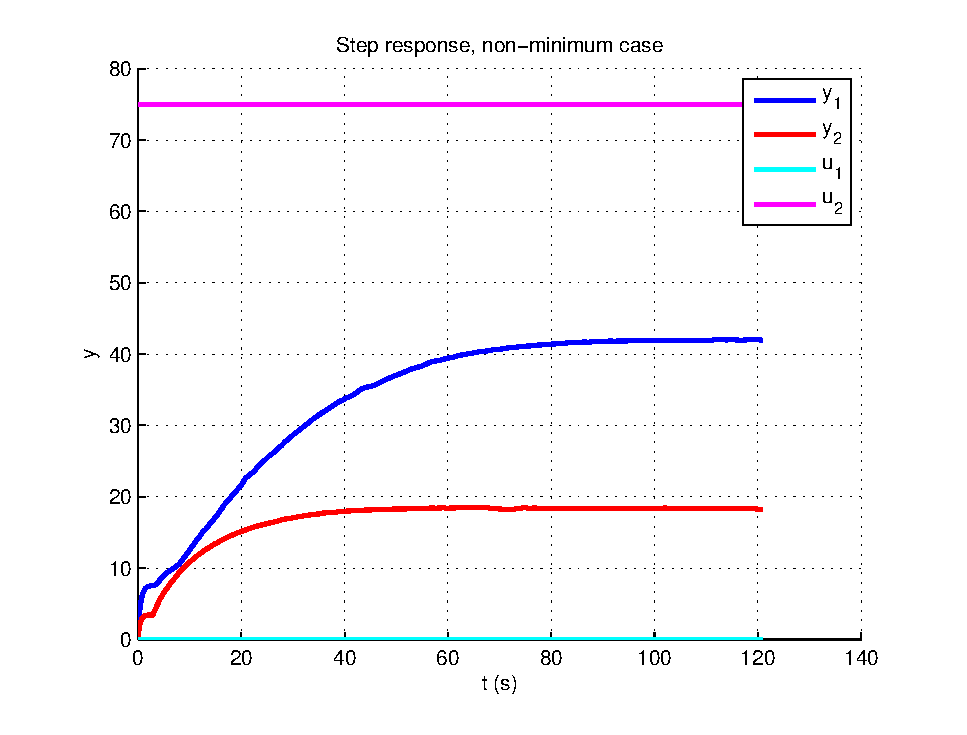
\includegraphics[width=\columnwidth]{fig/steprepnonmin75_0.eps}
                \caption{$u_1 = 0\%, u_2 = 75\%$}
        \end{subfigure}
        \caption{Step response from one input at a time \\ for the non-minimum phase case} 
        \label{steprepnonmin}
\end{figure}


% \subsubsection{Exercise}

Our objective now is to determine two inputs ($u_1, u_2$) in order to reach $60\%$ of full tank in tank $1$ and $2$.

Once the values for each parameters $a_{1 \leq i \leq 4}$ and $k_{1,2}$ are known, the equilibrium system from exercice 2.1.2 can be solved in order to find the values of $h_3^0,h_4^0,u_1,u_2$ (inputs are $h_1^0,h_2^0$).  

The system is the following:
$$
    \footnotesize
\left[
    \begin{array}{cccc}
        \gamma_1 k_1 & 0 & a_3 \sqrt{2g} & 0 \\
        0 & \gamma_2 k_2 & 0 & a_4 \sqrt{2g} \\
        0 & (1-\gamma_2) k_2 & -a_3 \sqrt{2g} & 0 \\
        (1-\gamma_2) k_1 & 0 & 0 & -a_4 \sqrt{2g} \\
    \end{array}
\right]
\left[
    \begin{array}{c}
        u1 \\ u2 \\ \sqrt{h_3^0} \\ \sqrt{h_4^0}
    \end{array}
\right]
=
\left[
    \begin{array}{c}
        a_1 \sqrt{2gh_1^0} \\
        a_2 \sqrt{2gh_2^0} \\
        0 \\
        0 \\
    \end{array}
\right]
$$

Therefore solving this linear with $h_1^0$ and $h_2^0$ as parameters compute the values of $u_1$ and $u_2$. 
Using this method with the two sets of parameters (Minimum and non-minimum case) leads to the results display in Figure \ref{manualcontrol}.

The transient time is reported in the following table:

\begin{center}
    \footnotesize
\begin{tabular}{|cc|}
    \hline
    \multicolumn{2}{|c|}{Transient time} \\
    \hline
    Mininum case & $98$s \\
    Non-mininum case & $55$s \\
    \hline
\end{tabular}
\end{center}

\begin{figure}[h!t]
        \centering
        \begin{subfigure}[b]{0.45\columnwidth}
                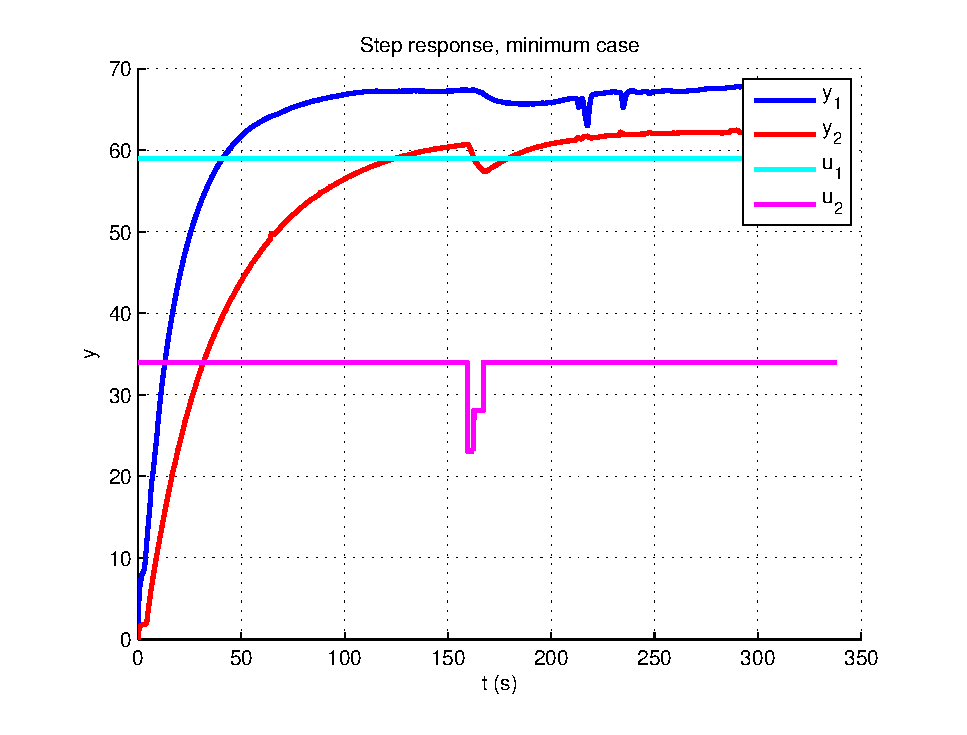
\includegraphics[width=\columnwidth]{fig/manualcontrolmin.eps}
                \caption{$u_1 = 59\%, u_2 = 34\%$ \\ $h_1^0 = h_2^0 = 15cm$}
        \end{subfigure}
        \begin{subfigure}[b]{0.45\columnwidth}
                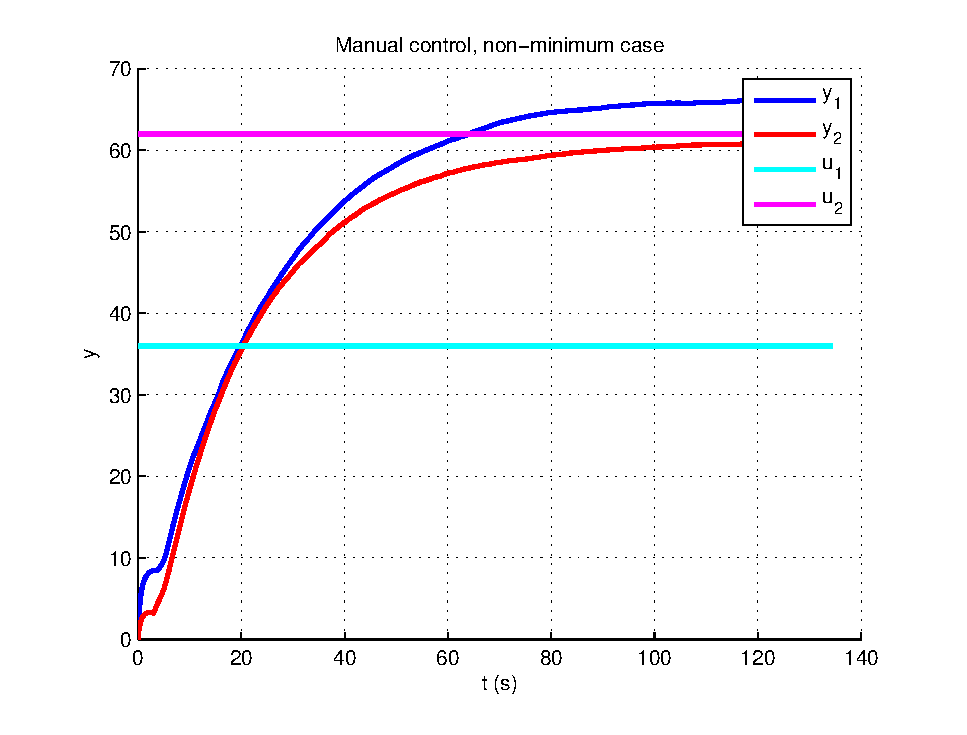
\includegraphics[width=\columnwidth]{fig/manualcontrolnonmin.eps}
                \caption{$u_1 = 36\%, u_2 = 62\%$ \\ $h_1^0 = h_2^0 = 15cm$}
        \end{subfigure}
        \caption{Manual control of $h_1^0, h_2^0$}
        \label{manualcontrol}
\end{figure}



The two curves do not merge after the transient time. Indeed, the two capter present different offset (\emph{i.e} $h_1 = 0$ do not lead to exactly $y_1 = 0$).
However this offset is constant for each capter and verification do lead to the same level in both tank.


% \subsubsection{Exercise}

From the previous exercises, we can formulate the following conclusions:
\begin{shortitemize}
\item The coupling exists in both case,
\item The coupling is more important in the non-minimum phase case ($3.9 \geq 2.9$ and $4.6 \geq 2.2$)
\item The transient time is smaller in the non-minimum phase case (for manual control). This result seems surprising. Indeed, we would have expect to find a faster system in the minimum phase case (since filling the lower tanks is mostly made by emptying the upper tanks in the non-minimum phase case).
\end{shortitemize}


% 
% \section{Calculation of controllers}
% 
% \setcounter{subsection}{1}
% \subsubsection{Exercise}
\paragraph{Minimum phase model}

The transfer matrix $G_{mp}(s)$ is:

$$G_{mp}(s) = \left(\begin{array}{cc} 
    \frac{.035}{s + .056} & \frac{.00046}{s^2 + .082 s + .0015} \\
    \\
    \frac{ .00044}{  s^2 + .073 s + .0011} & \frac{.030}{s + .052} \\
\end{array}\right)$$


Poles and zeros of the elements are given in the following table:

$$
\text{Poles}(G_{mp,i,j}(s)) = \left(\begin{array}{cc} -.056 & \left(\begin{array}{c} -.056\\ -.026 \end{array}\right) \\ \left(\begin{array}{c} -.052\\ -.021 \end{array}\right) & -.052 \\ \end{array}\right)
$$

$$\text{Zeros}(G_{mp,i,j}(s)) = \emptyset $$

\paragraph{Non-minimum phase model}

The transfer matrix $G_{nmp}(s)$ is:

$$G_{nmp}(s) = \left(\begin{array}{cc} 
    \frac{.021}{s + .051} & \frac{.0026}{s^2 + .14 s + .0044} \\
    \\
    \frac{ .0032}{ s^2 + .14 s + .0043} & \frac{.018}{s + .047} \\
\end{array}\right)$$

Poles and zeros of the elements are given in the following table:


$$\text{Poles}(G_{nmp,i,j}(s)) = 
\left(\begin{array}{cc} -.051 & \left(\begin{array}{c} -.086\\ -.051 \end{array}\right) \\ \left(\begin{array}{c} -.091\\ -.047 \end{array}\right) & -.047 \\ \end{array}\right)
$$

$$\text{Zeros}(G_{nmp,i,j}(s)) = \emptyset $$

% \setcounter{subsection}{-1}
% 
% \section{Laboratory occasion 2}
% 
% In the following section we will test our decentralized controllers and analyse the impact of externals perturbations (pouring a cup of water in one of the lower tank and opening an extra outlet in one of the upper tanks).

Our controller are used in small deviation cases ($\approx 5\%$) around the equilibrium point (set as $50\%$ for each pump). 

For Figures \ref{min_dyn_fig} to \ref{nonmin_glover_fig}, each of the following experiment is done:
\begin{shortitemize}
    \item Step response relative to input 1,
    \item Cup of water in tank 1,
    \item Extra outlet in tank 3.
\end{shortitemize}
\subsection{Decentralized control}


\subsubsection{Exercise}

We want to design a lead-lag controller which eliminates the static control error for a step response in the reference signal.

The controller transfer function is the following:

$$ F(s) = K \frac{\tau_D s + 1}{\beta \tau_D s + 1} \frac{\tau_I s + 1}{\tau_I s + \gamma}$$

We want to fulfill the following criteria:
\begin{itemize}
 \item Phase margin of $30^{\circ}$ at the cross-over frequency $\omega_c = 0.4$ rad/s.
 \item No static control error for a step response 
\end{itemize}

\subsubsection{Exercise} 

The main differences between the minimum phase case and the non-minimum phase case using a decentralized controller are:
\begin{shortitemize}
    \item The non-minimum phase system is much slower (both for step response and disturbance rejection);
    \item The step response of the non-minimum phase system starts by decreasing its value (wrong direction!);
    \item Disturbances on the top tanks have more impact on the non-minimum phase system (whereas the perturbation on the lower tanks have a similar impact on both systems).
\end{shortitemize}



% 
% 
\subsection{Robust control}

\subsubsection{Exercise}

Since $G_d(s) = \frac{10}{s+1}$, the cross-over frequency is $w_c = 10$ rad/s.

We have the following result:

$$\forall \omega < \omega_c, |Gd(j\omega)| >1$$

Control action is needed at least for $\omega \in [0,\omega_c]$.

Here, we will try to design $F_y$ in such a way that:
$$L(s) = F_y G \approx \frac{\omega_c}{s}$$

\paragraph{Unproper feedback}
Let:
$$F_y = G^{-1} \frac{\omega_c}{s} = \frac{200 s^3 + 4200 s^2 + 84000 s + 80000}{160000 s}$$

This controller has $3$ zero and $1$ pole. Thus, it is not proper. However -- using \texttt{Matlab} -- we can plot the step response of the system and the step response to a step perturbation (see Figure \ref{stepNonProper}).

\begin{figure}[h!t]
    \centering
    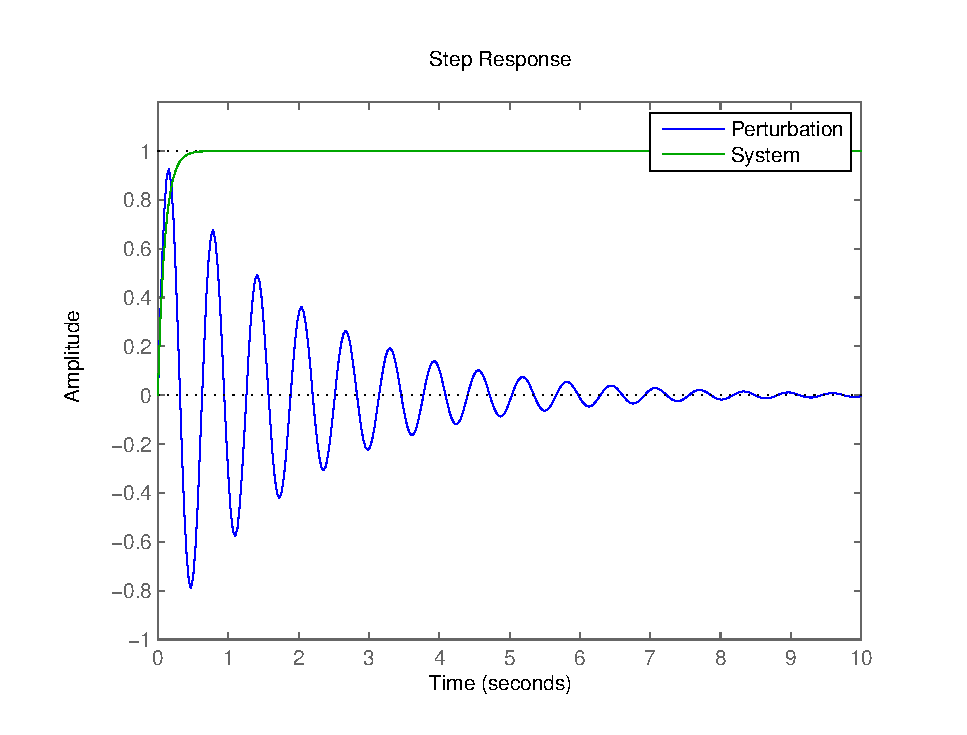
\includegraphics[width=\linewidth]{fig/stepNonProper421.eps}
    \caption{Non-proper step response of the system}
    \label{stepNonProper}
\end{figure}

We can see that even if the performance are poor (Error static $\leq 5\%$ for $t \geq t_d = 7$ s) we still have an attenuation of the perturbation and a step response of good quality.

\paragraph{Proper feedback}
Assuming that this controller is the one we want to implement, we need to design it in a proper way. For now, it has $3$ zeros and $1$ pole. Therefore it is needed to add two more poles.

Let:
$$F_y(s) = G^{-1}\frac{\omega_c}{s(s+p_1)(s+p_2)}$$

We need to choose $p_{1,2}$ in order to not change the system performance two much.

We use the following criteria:

\begin{shortitemize}
    \item $p_1 = p_2$
    \item $p_1$ and $p_2$ take action after $\omega_c$ 
\end{shortitemize}

Let's pick $p_1 = p_2 = p = 100\omega_c$. In order to have the same bode diagram for $\omega < \omega_c$, we need to translate the gain curve with a gain of $p^2$. Figure \ref{bodeProper421} shows the bode diagram of $L(s) = F_y(s) G(s)$ (we can see that $\forall \omega < \omega_c, |L_{proper}|_{dB} \approx |L_{unproper}|_{dB}$). Figure \ref{stepProper421} shows that the step response to a perturbation with $L_{proper}$ is almost the same than with $L_{unproper}$.

\begin{figure}[h!b]
    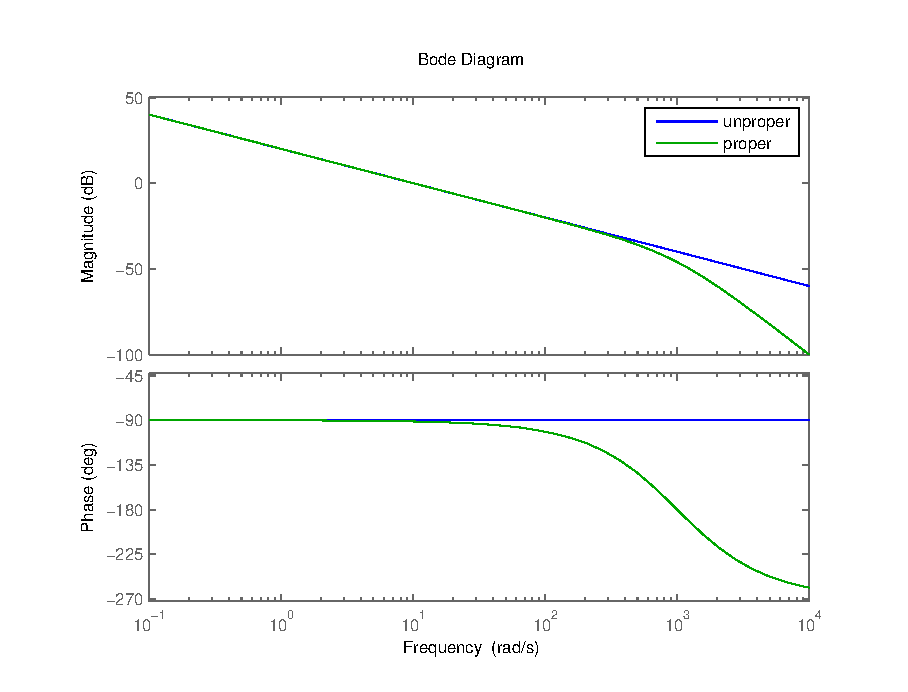
\includegraphics[width=\columnwidth]{fig/bodeProper421.eps}
    \caption{Bode diagram of $L(s)$ with the proper \& unproper $F_y$} 
    \label{bodeProper421}
\end{figure}

\begin{figure}[h!b]
    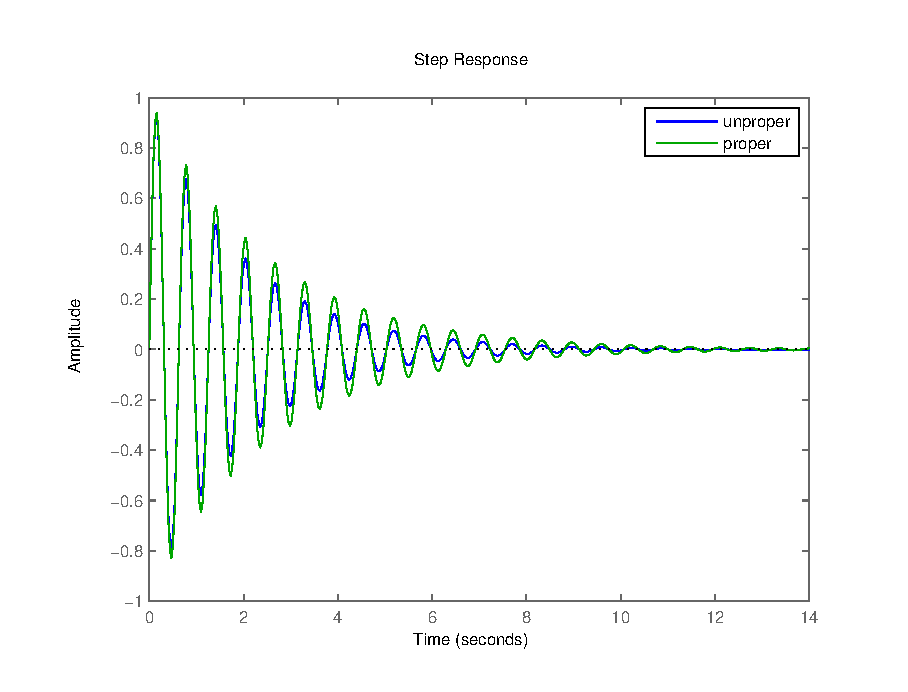
\includegraphics[width=\columnwidth]{fig/stepProper421.eps}
    \caption{Step response of the system with the proper \& unproper $F_y$} 
    \label{stepProper421}
\end{figure}


\subsubsection{Exercise} 

Using Glover-MacFarlane controllers lead to a huge improvement of the controlled system:
\begin{shortitemize}
    \item All time are reduced (at least by a factor 2)
    \item Overshoots are decreased (at least by a factor 5)
    \item The step responses (non-minimum case) do not go in the wrong direction
\end{shortitemize}

\subsubsection{Exercise} 

The main differences between the minimum phase case and the non-minimum phase case using Glover-MacFarlane controllers are (differencies are rather similar as the one using the decentralized controllers):
\begin{shortitemize}
    \item The non-minimum phase system is much slower (both for step response and disturbance rejection);
    \item Disturbances on the top tanks have more impact on the non-minimum phase system (whereas the perturbation on the lower tanks have a similar impact on both systems).
\end{shortitemize}



% 
% \vspace{.5cm}
\hrulefill
\vspace{.5cm}

\begin{bfseries}
\emph{Conclusion} -- Pouet.
\end{bfseries}


\end{document}
